\section{Durchführung}
\subsection{Versuchsaufbau}
Der für den Veruch genutzte Aufbau ist in Abb.\ref{aufbau} schematisch dargestellt.
\begin{figure}
  \centering
  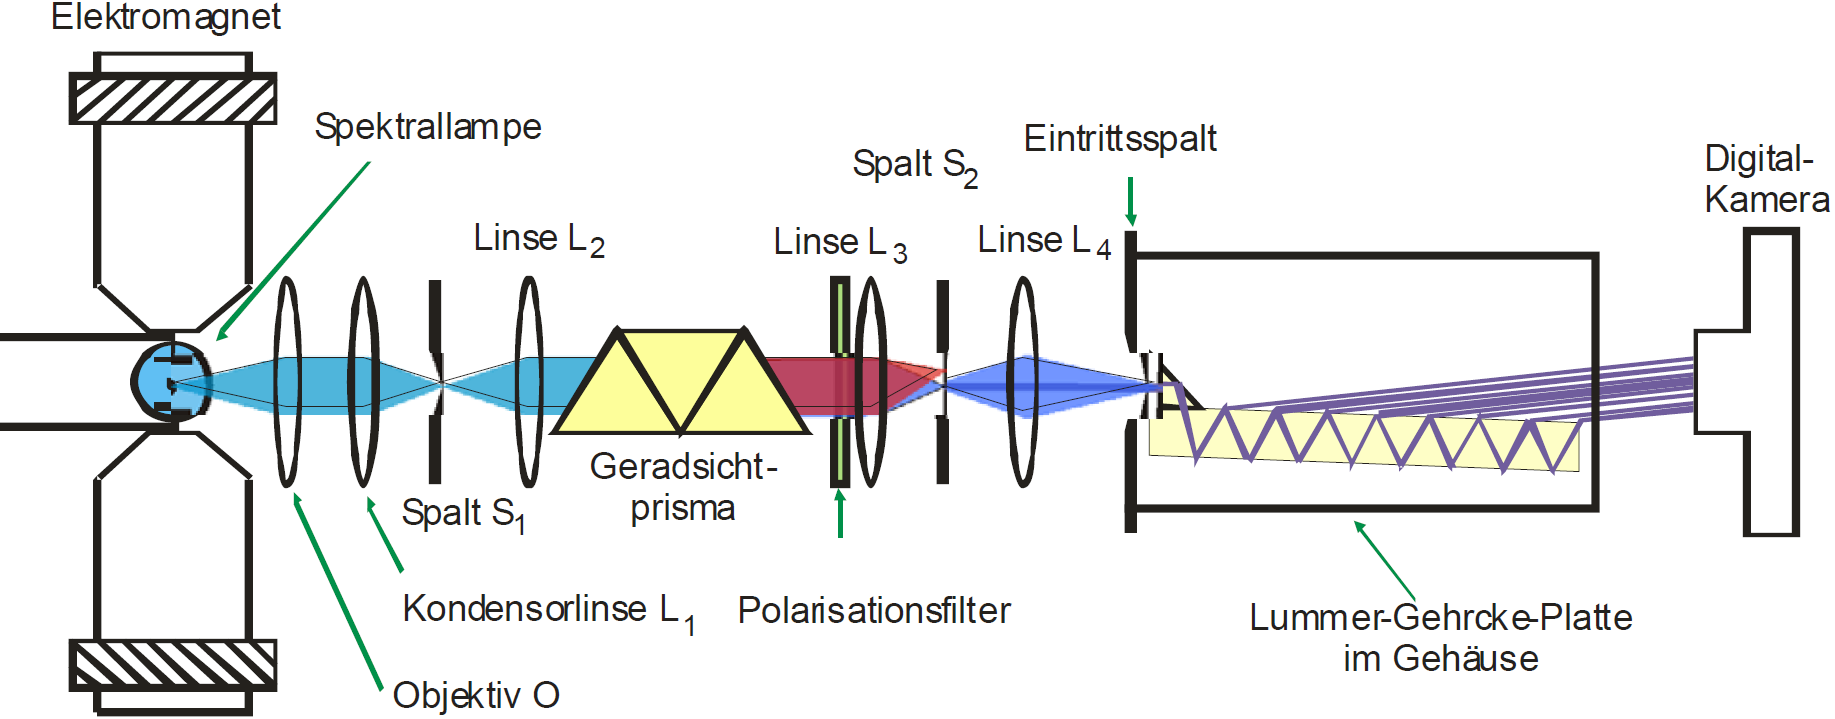
\includegraphics[width=0.9\textwidth]{Bilder/aufbau.png}
  \caption{Schematische Darstellung des im Versuch genutzten Aufbaus \cite{anleitung}.}
\end{figure}
Als Lichtquelle zur Untersuchung der Spektrallinien dient eine Cadmiumdampflampe die in einem Elektromagneten platziert ist, welcher sich über seine Stromversorgung steuern lässt. Das Licht wird mit einem Objektiv und einer Kondensorlinse auf einen Spalt fokussiert. Mit einer zweiten Linse wird dann ein möglichst paralleles Lichtbündel auf ein Geradsichtprisma gelenkt, welches das Licht in seine Spektrallinien aufteilt. Ein Polarisationsfilter erlaubt die Untersuchung der Polarisationseigenschaften der Strahlung. Nach fokussierung durch eine dritte Linse fällt das Licht auf einen weiteren Spalt der auf einer senkrecht zur Richtung der optischen Achse verlaufenden Schiene befestigt ist und es somit erlaubt es die gewünschte Spektrallinie zu isolieren. Diese wird danach ein letztes mal mit einer Linse fokussiert und trifft dann auf eine Lummer-Gehrke-Platte.
Bei der Lummer-Gehrke-Platte handelt es sich um ein optsches Instrument, welches Interferenz an planparallelen Platten ausnutzt um ein sehr hohes Auflösungsvermögen zu erzielen. Das Licht wird durch ein Prisma so auf ein paar planparallele Platten gelenkt, dass bei jeder Reflektion nur ein geringer Teil der Strahlung transmittiert wird. Dieser geringe Anteil des austretenden Lichts kann dann gemäß der Bedingung
\begin{equation}
2d\cos{\theta}=n\lambda\,,
\end{equation}
wobei d die Dicke der Platte und $\lambda$ die Wellenlänge des Lichts ist, mit anderen Strahlenbündeln interferieren. Dies erlaubt es für monochromatisches Licht aus dem Gangunterschied der Maxima die Wellenlänge zu bestimmen. Des Weiteren ist es wird beim Einschalten eines externen Magnetfelds, wegen der sich ändernden Wellenlänge, der Abstand der Maxima um $\updelta s$ verschoben.
Das Auflösungsvermögen einer Lummer-Gehrke-Platte ist gegeben durch
\begin{equation}
A=\frac{L}{\lambda}\left(n^2-1\right)\,,
\label{eq:auf}
\end{equation}
wobei L die Länge der Platte und n der Brechungsindex ist. Es existiert auch eine maximale Wellenlängendifferenz die notwendig ist, damit sich zwei Wellenlängen nicht überlagern. Dieses Dispersionsgebiet ist gegeben durch:
\begin{equation}
\upDelta \lambda_\text{D}=\frac{\lambda^2}{2d}\sqrt{\frac{1}{n^2-1}}\,.
\label{eq:disp}
\end{equation}\\
Das Interferenzmuster der Lummer-Gehrke-Platte lässt sich mit einer Digitalkamera aufnehmen.
\subsection{Versuchsdurchführung}
Zu Beginn des Versuchs muss der Elektromagnet durch mit einer Hall-Sonde geeicht werden. Hierzu wird der Betriebsstrom stückweise erhöht und jeweils die Feldstärke gemessen.\\
Anschließend wird mit dem Aufbau ein Interferenzmuster erzeugt welches in der Kamera gut sichtbar ist. Es wird eine rote Linie ($\lambda=643{,}8\,\si{\nm}$) und eine eine blaue Linie ($\lambda=480\si{\nm}$) jeweils mit und ohne Magnetfeld für verschiedene Polarisationsrichtungen untersucht.
